\section{Dataset Description and Data Capture}
\label{sec:data_capture}

\subsection{Tissue-Mimicking Phantoms}
The experiments were conducted on protein-doped agar phantoms.
The agar (manufacturer, product, and grade: XXXX) provided a solid, tissue-mimicking
medium, while egg white (Liquid Egg Whites, GymBeam Germany GmbH, Kempen, Germany) produced
a visible coagulation pattern after microwave heating. 
The recipe and fabrication procedure are provided in the Supplementary Material. 
The phantoms were cast in a 3D-printed mold and allowed to set at room temperature (22\,$^\circ$C) before use.

\subsection{Experimental Setup}
A custom 3D-printed holder was used to position the phantom, microwave ablation
(MWA) antenna, ultrasound probe, and four fiber-optic temperature probes for punctual temperature monitoring.
The
holder includes guides for repeatable probe placement and a support for the
ultrasound probe. Before each trial, the antenna path was made using a 12 Gauge biopsy
needle to reduce displacement of the phantom and temperature probes during antenna insertion. 
The antenna was inserted to a consistent depth of (XX\,mm) using a depth mark. The four
temperature probes were positioned to the right of the antenna, at a
perpendicular distance of (XX\,mm) and an in-plane distance of (XX\,mm)-
The sensors were numbered 1–4 starting at the upper left and arranged symmetrically around the antenna active zone.
MWA was delivered using a 2.45 GHz water-cooled microwave ablation system (Saberwave ECO-200G, ECO Medical Technology, Nanjing, China) and an antenna.
The ultrasound images were acquired with a handheld US scanner (GE Vscan Air CL, GE HealthCare Technologies Inc, Chicago, United States of America) as video sequences with a frame rate of 30\,fps.
The scanner was connected to a tablet through its companion application (GE Vscan Air CL, GE HealthCare Technologies Inc, Chicago, United States of America) via bluetooth.
Because the application limits individual video recordings to 10 seconds, the display was recorded using the tablets screen-capture software to retain the full ablation session.
 
The four fiber-optic temperature probes  were connected to a thermometer (COMEM Optocon GmbH, Dresden, Germany) recording at 250 ms intervals.
The thermometer was connected to a computer via USB for temperature logging using software (FOTEMP ASSISTANT 2, Micronor Sensors Inc., Ventura, United States of America).
Temperature readings were recorded at intervals of 250\,ms. 

\begin{figure*}[t]
    \begin{minipage}[t]{0.68\textwidth}
        \centering
        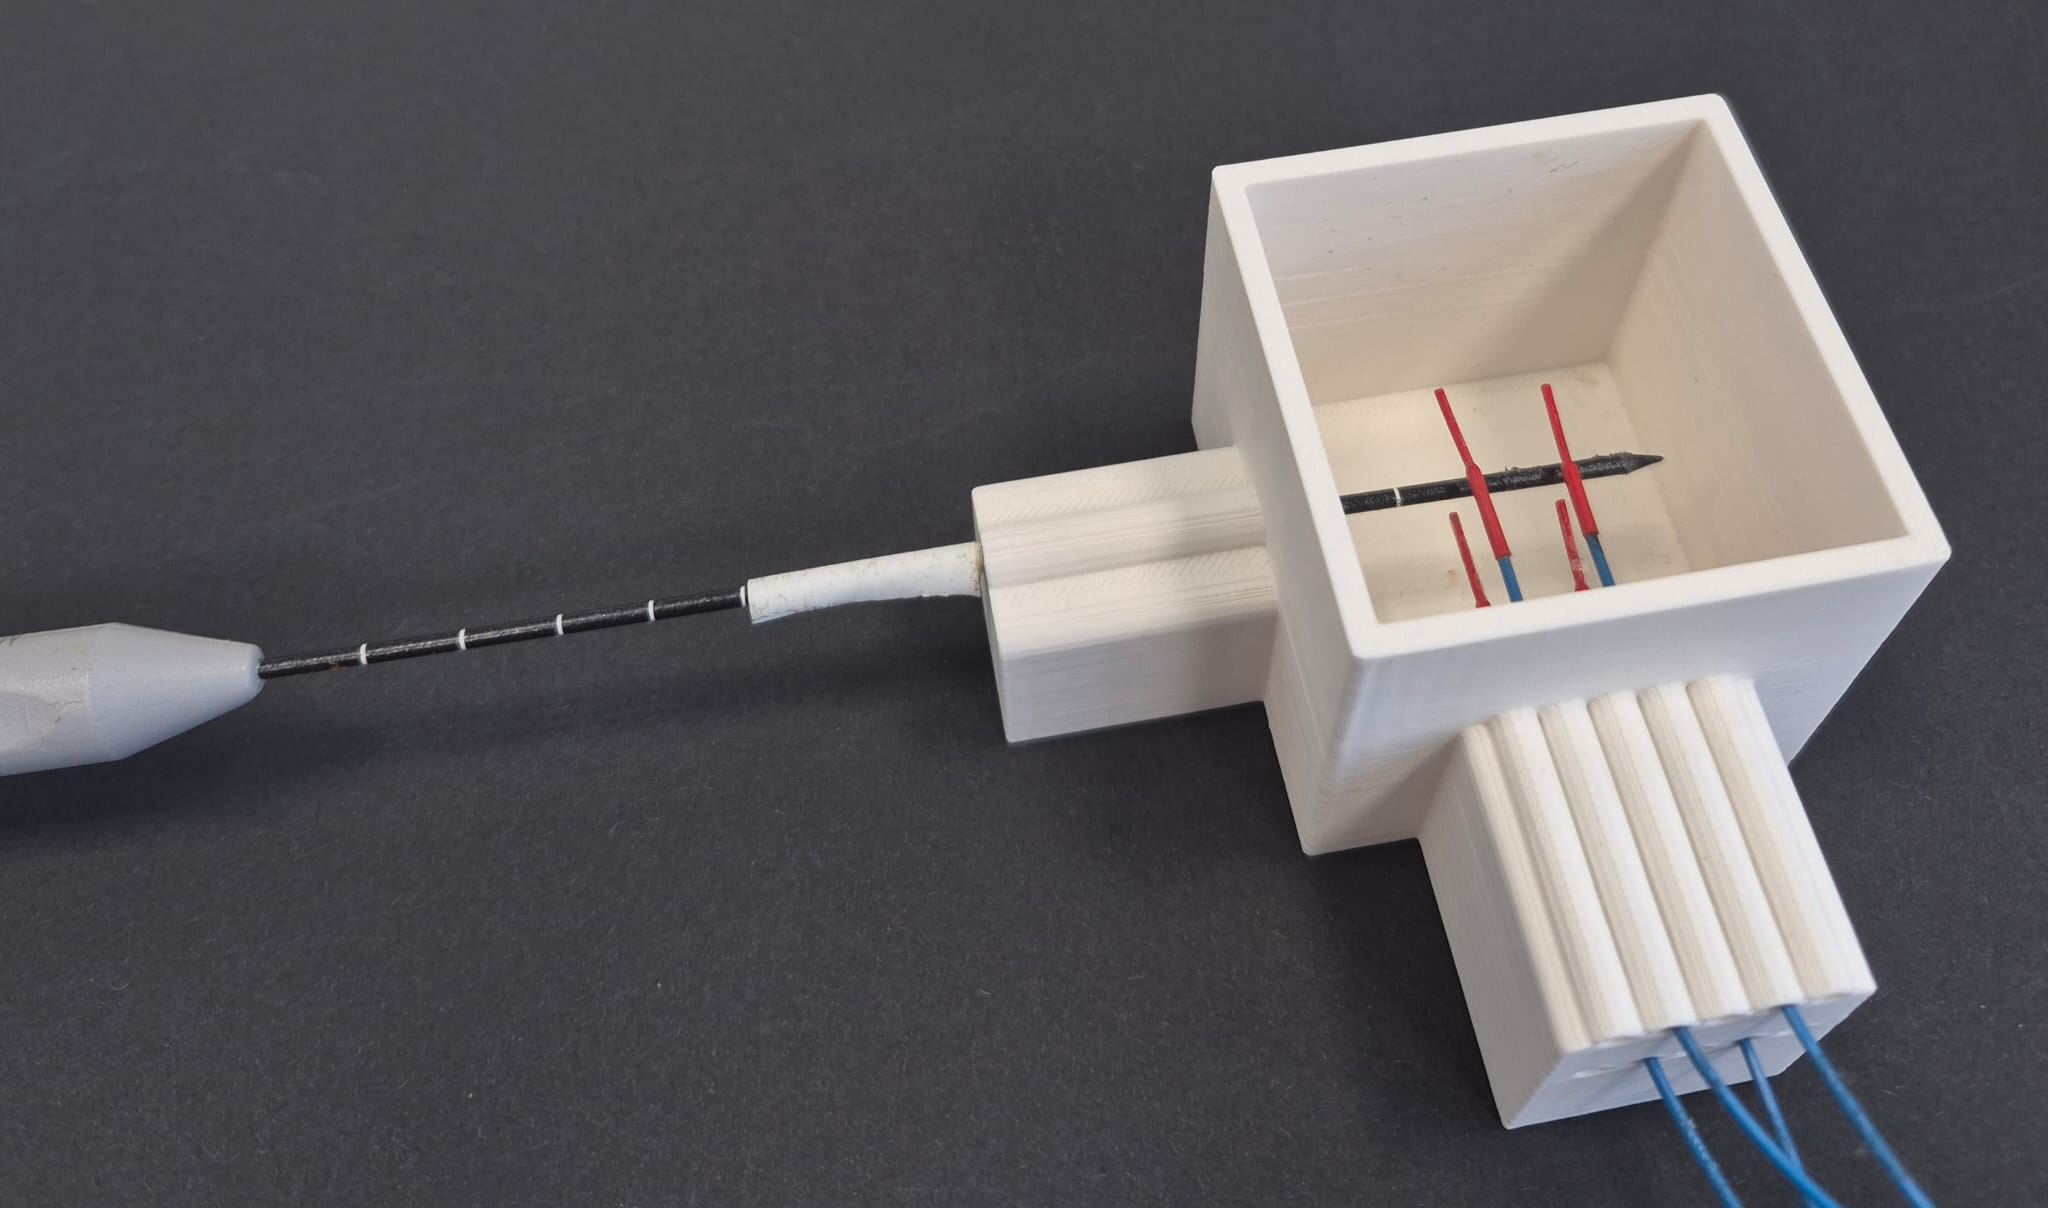
\includegraphics[width=\linewidth]{../experiment/MWA_Projekt_Bilder/messaufbau.jpeg}
        \centerline{(a) Phantom and probe guides}
    \end{minipage}\hfill
    \begin{minipage}[t]{0.3\textwidth}
        \centering
        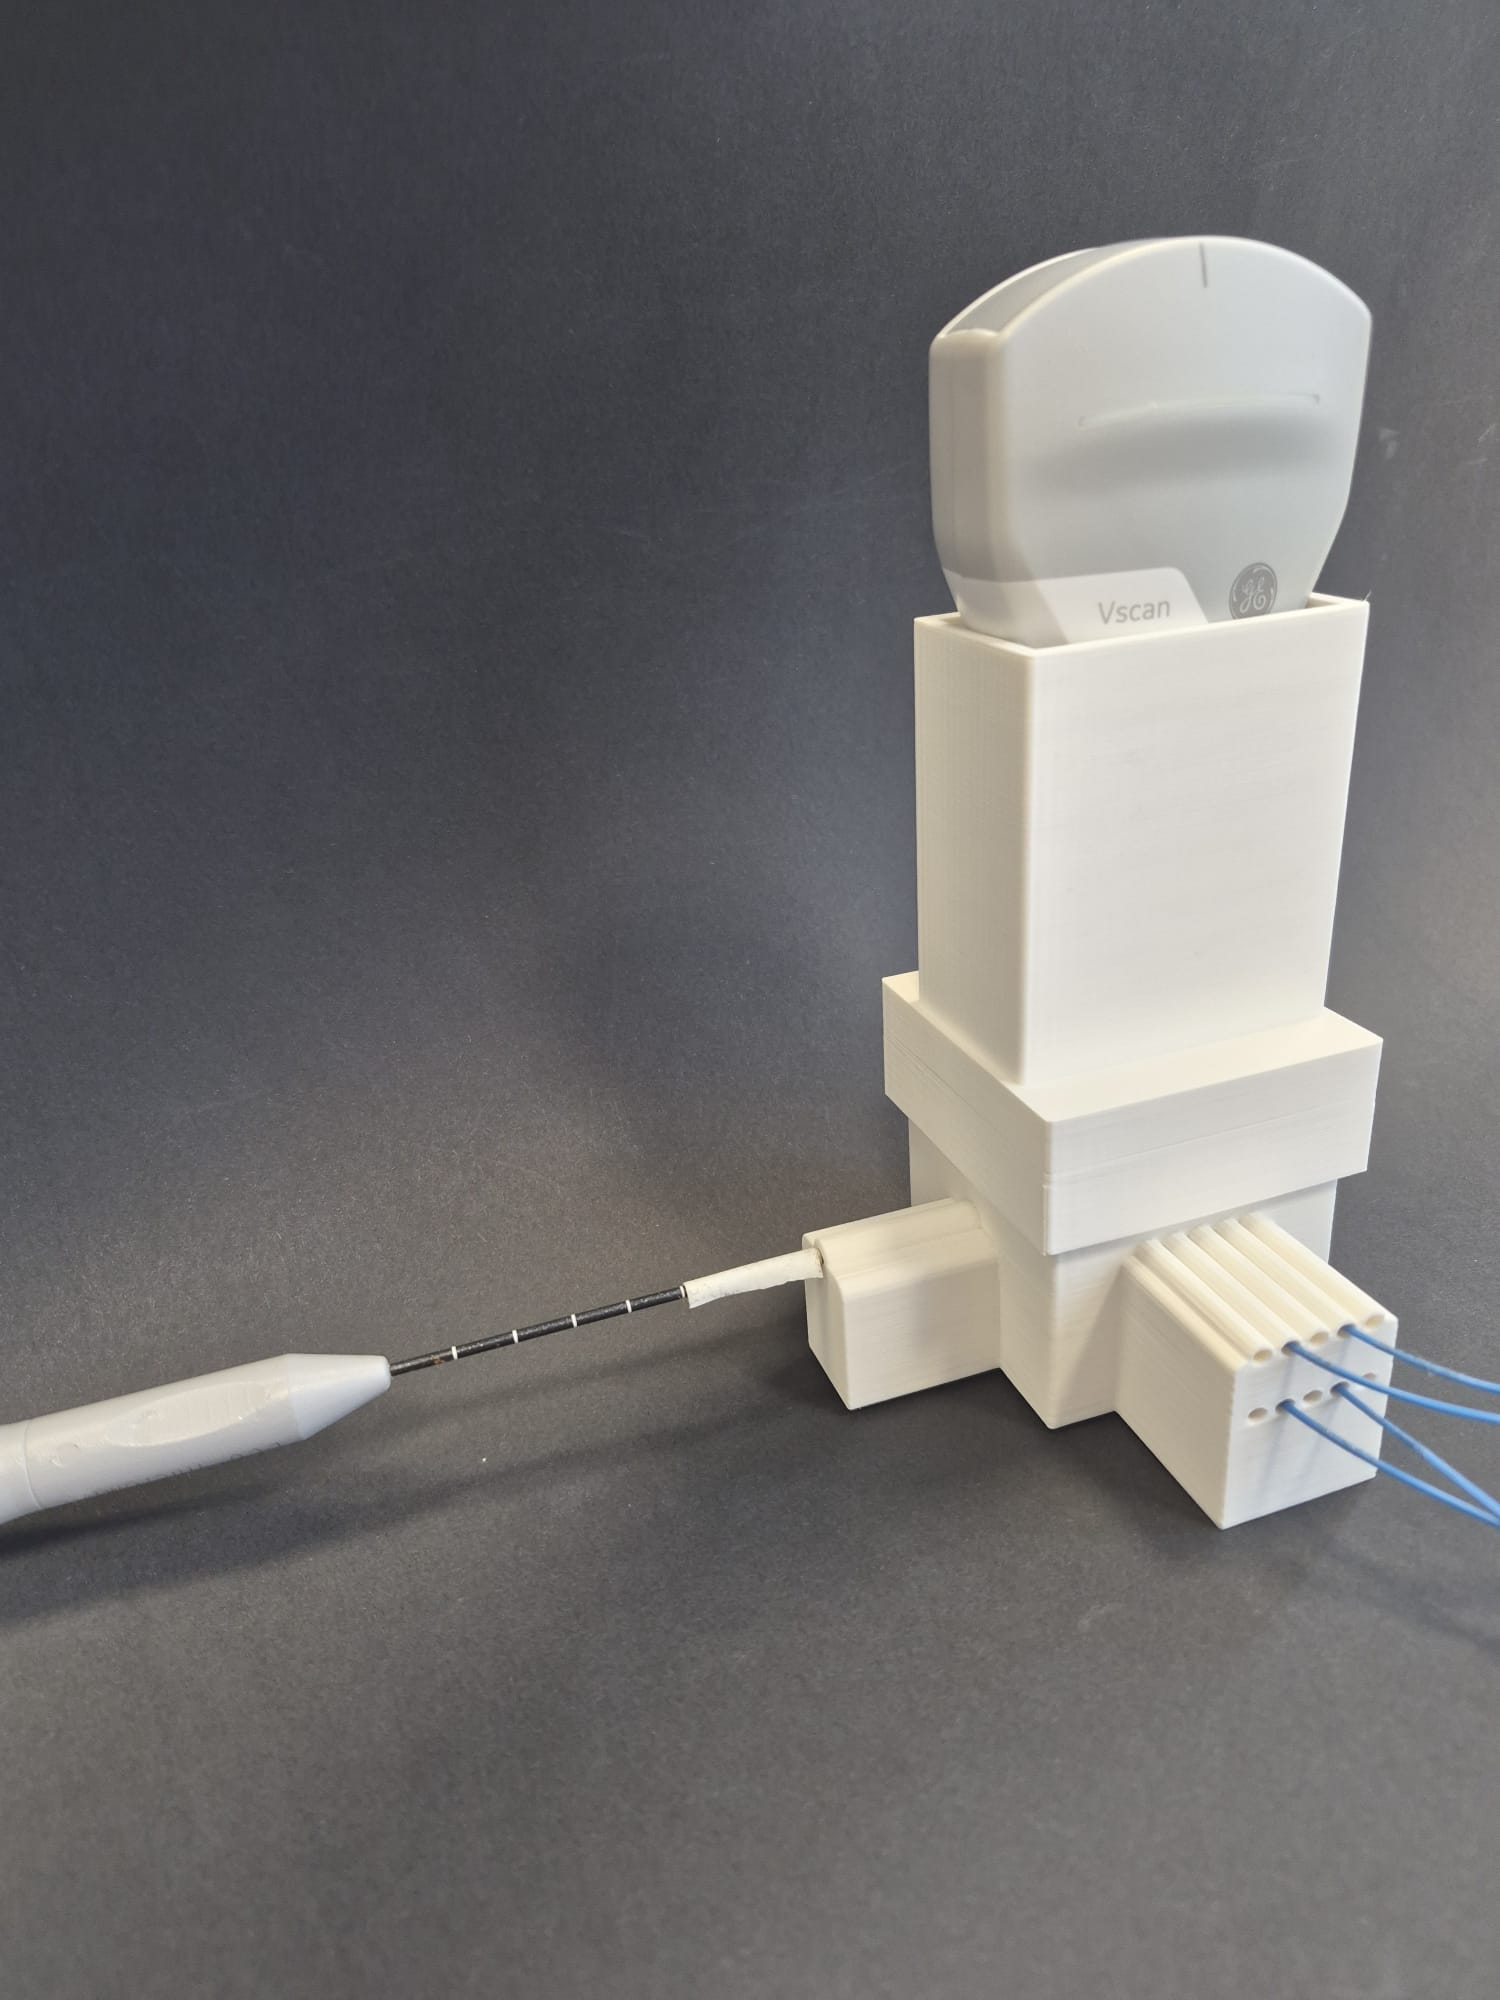
\includegraphics[width=\linewidth]{../experiment/MWA_Projekt_Bilder/gesamtaufbau.jpeg}
        \centerline{(b) Assembled acquisition setup}
    \end{minipage}
    \caption{Custom experimental arrangement for acquiring ultrasound video
    and temperature measurements during MWA. The phantom, antenna, temperature
    probes, and ultrasound probe are held in a 3D-printed fixture.}
    \label{fig:experimental_setup}
\end{figure*}

\subsection{Ablation and Data Acquisition}
Ultrasound video and temperature logging were initiated at the start of each MWA treatment and continued during heating. Each ablation lasted 10 minutes
The nominal power settings represented in the collected trials ranged from 25\,W to 50\,W in 5\,W increments. 
The four fiber-optic probes provided point-wise temperature measurements, which were paired with the corresponding ultrasound video frames for supervised temperature estimation. Figure
\ref{fig:representative_bmode} shows a representative B-mode frame with the
antenna track and temperature-probe locations visible in the phantom.

\begin{figure}[t]
    \centering
    \includegraphics[width=\columnwidth]{\detokenize{../experiment/MWA_Projekt_Bilder/US 4 Startbild.jpeg}}
    \caption{Representative B-mode image of the phantom showing the MWA
    antenna track and the four temperature-probe locations.}
    \label{fig:representative_bmode}
\end{figure}

The dataset comprises 15 phantom subjects and 53,878 sequence samples from
multiple trials with different power settings and phantom compositions.
These data represent the heating phase; a post-ablation cooling phase was not
recorded.

%das gehört nicht in den aufbau
The measurements provide
temperature labels at the probe locations rather than a directly measured
spatial temperature field. Consequently, spatial temperature maps predicted
by the models are inferred from ultrasound and point-wise thermometry, not
directly observed ground truth.
